\section{Scenario 2}\label{sec:scenario2}
Scenario two is shown on Figure \ref{fig:topigraphic}(a), where the line-of-sight distance is shown on Figure \ref{fig:topigraphic}(b).  
%% images for p controller
% s1_topographic_map.eps
% 
%s1_p_drone_theta_phi_optimal.eps
%s1_p_gs_theta_phi_optimal.eps
%s1_p_los_distance.eps
%s1_p_prx.eps

\begin{figure}[H]
\hfill
\subfigure[.]{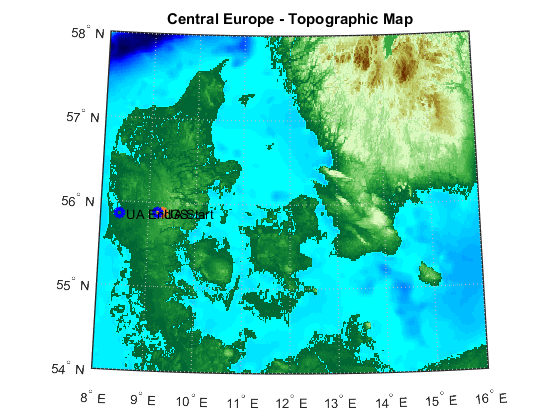
\includegraphics[scale=0.45]{figures/s2_topographic_map.png}}
\hfill
\subfigure[caption]{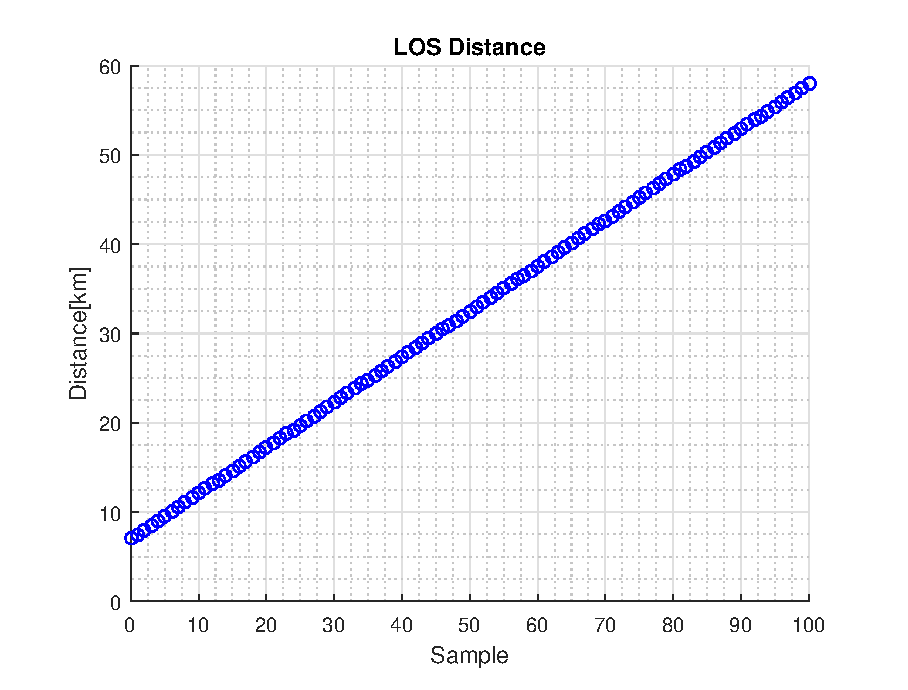
\includegraphics[scale=0.45]{figures/s2_pd_los_distance.eps}}
\hfill
\caption{caption}
\label{fig:topigraphic}
\end{figure}

\subsection{Drones}

Figure \ref{fig:s2_drones_p}, \ref{fig:s2_drones_pi}, \ref{fig:s2_drones_pd} and \ref{fig:s2_drones_pid}.
\begin{figure}[H]
\begin{minipage}[t]{0.45\textwidth}
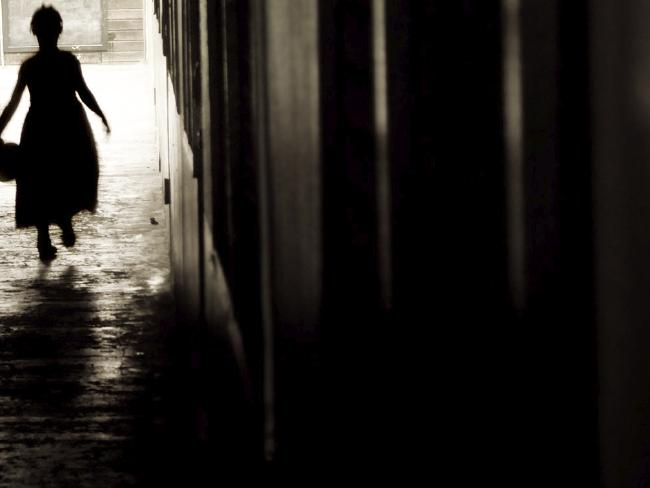
\includegraphics[width=\linewidth]{figures/randomfigure.jpg}
\caption{p}
\label{fig:s2_drones_p}
\end{minipage}
\hspace{\fill}
\begin{minipage}[t]{0.45\textwidth}
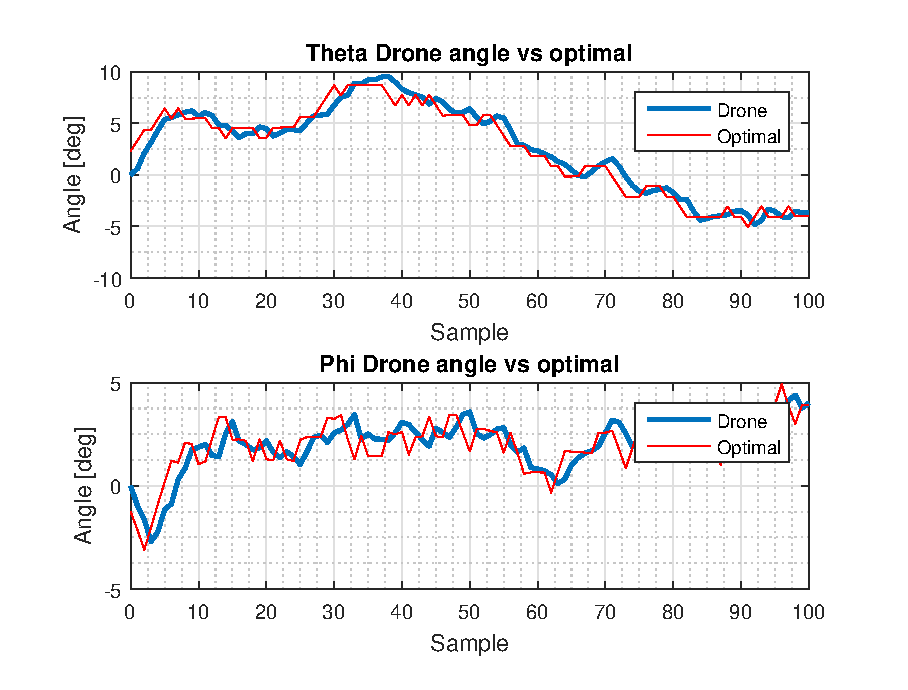
\includegraphics[width=\linewidth]{figures/s2_pi_drone_theta_phi_optimal.eps}
\caption{pi}
\label{fig:s2_drones_pi}
\end{minipage}

\vspace*{0.5cm} % (or whatever vertical separation you prefer)
\begin{minipage}[t]{0.45\textwidth}
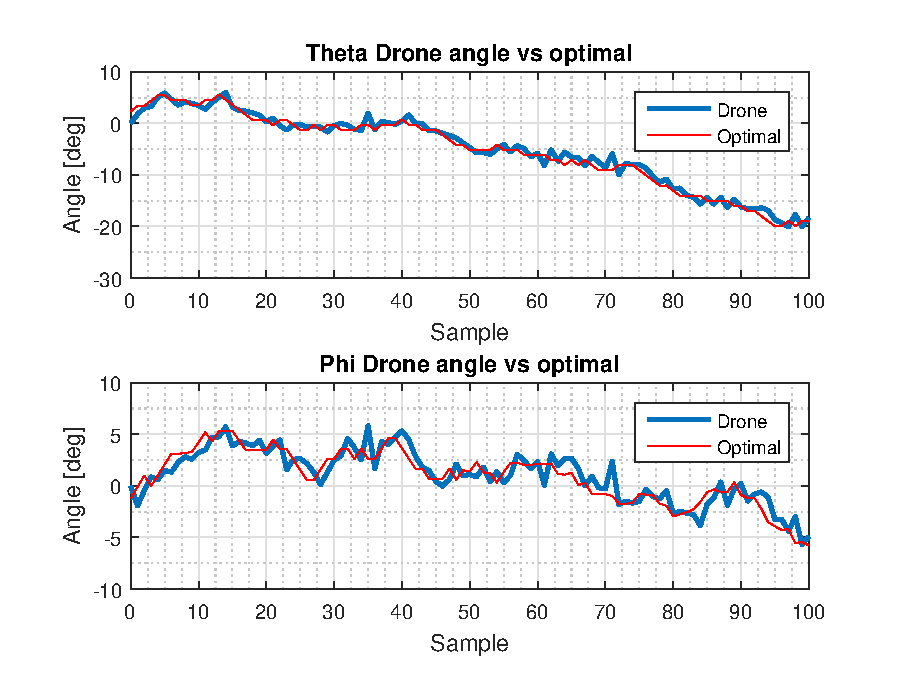
\includegraphics[width=\linewidth]{figures/s2_pd_drone_theta_phi_optimal.eps}
\caption{pd}
\label{fig:s2_drones_pd}
\end{minipage}
\hspace{\fill}
\begin{minipage}[t]{0.45\textwidth}
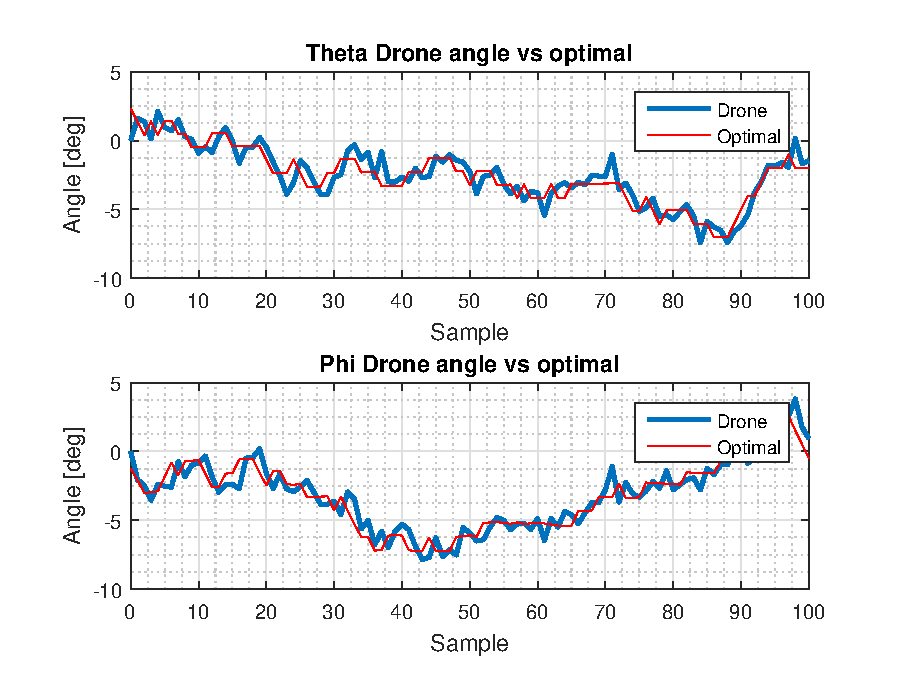
\includegraphics[width=\linewidth]{figures/s2_pid_drone_theta_phi_optimal.eps}
\caption{pid}
\label{fig:s2_drones_pid}
\end{minipage}

\end{figure}

\subsection{GS}
Figure \ref{fig:s2_gs_p}, \ref{fig:s2_gs_pi}, \ref{fig:s2_gs_pd} and \ref{fig:s2_gs_pid}

\begin{figure}[H]
\begin{minipage}[t]{0.45\textwidth}
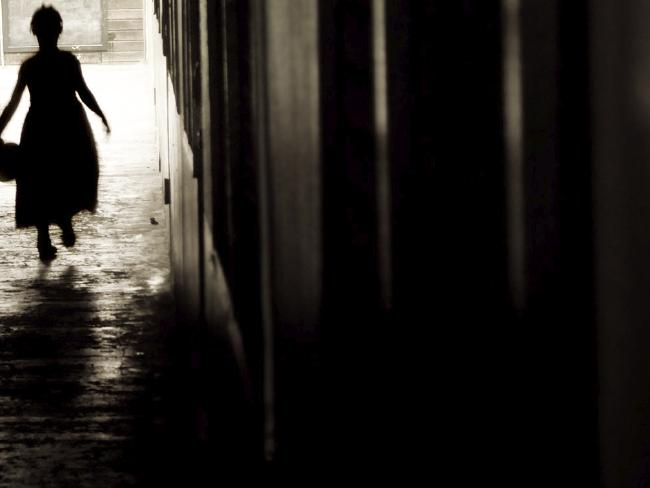
\includegraphics[width=\linewidth]{figures/randomfigure.jpg}
\caption{p}
\label{fig:s2_gs_p}
\end{minipage}
\hspace{\fill}
\begin{minipage}[t]{0.45\textwidth}
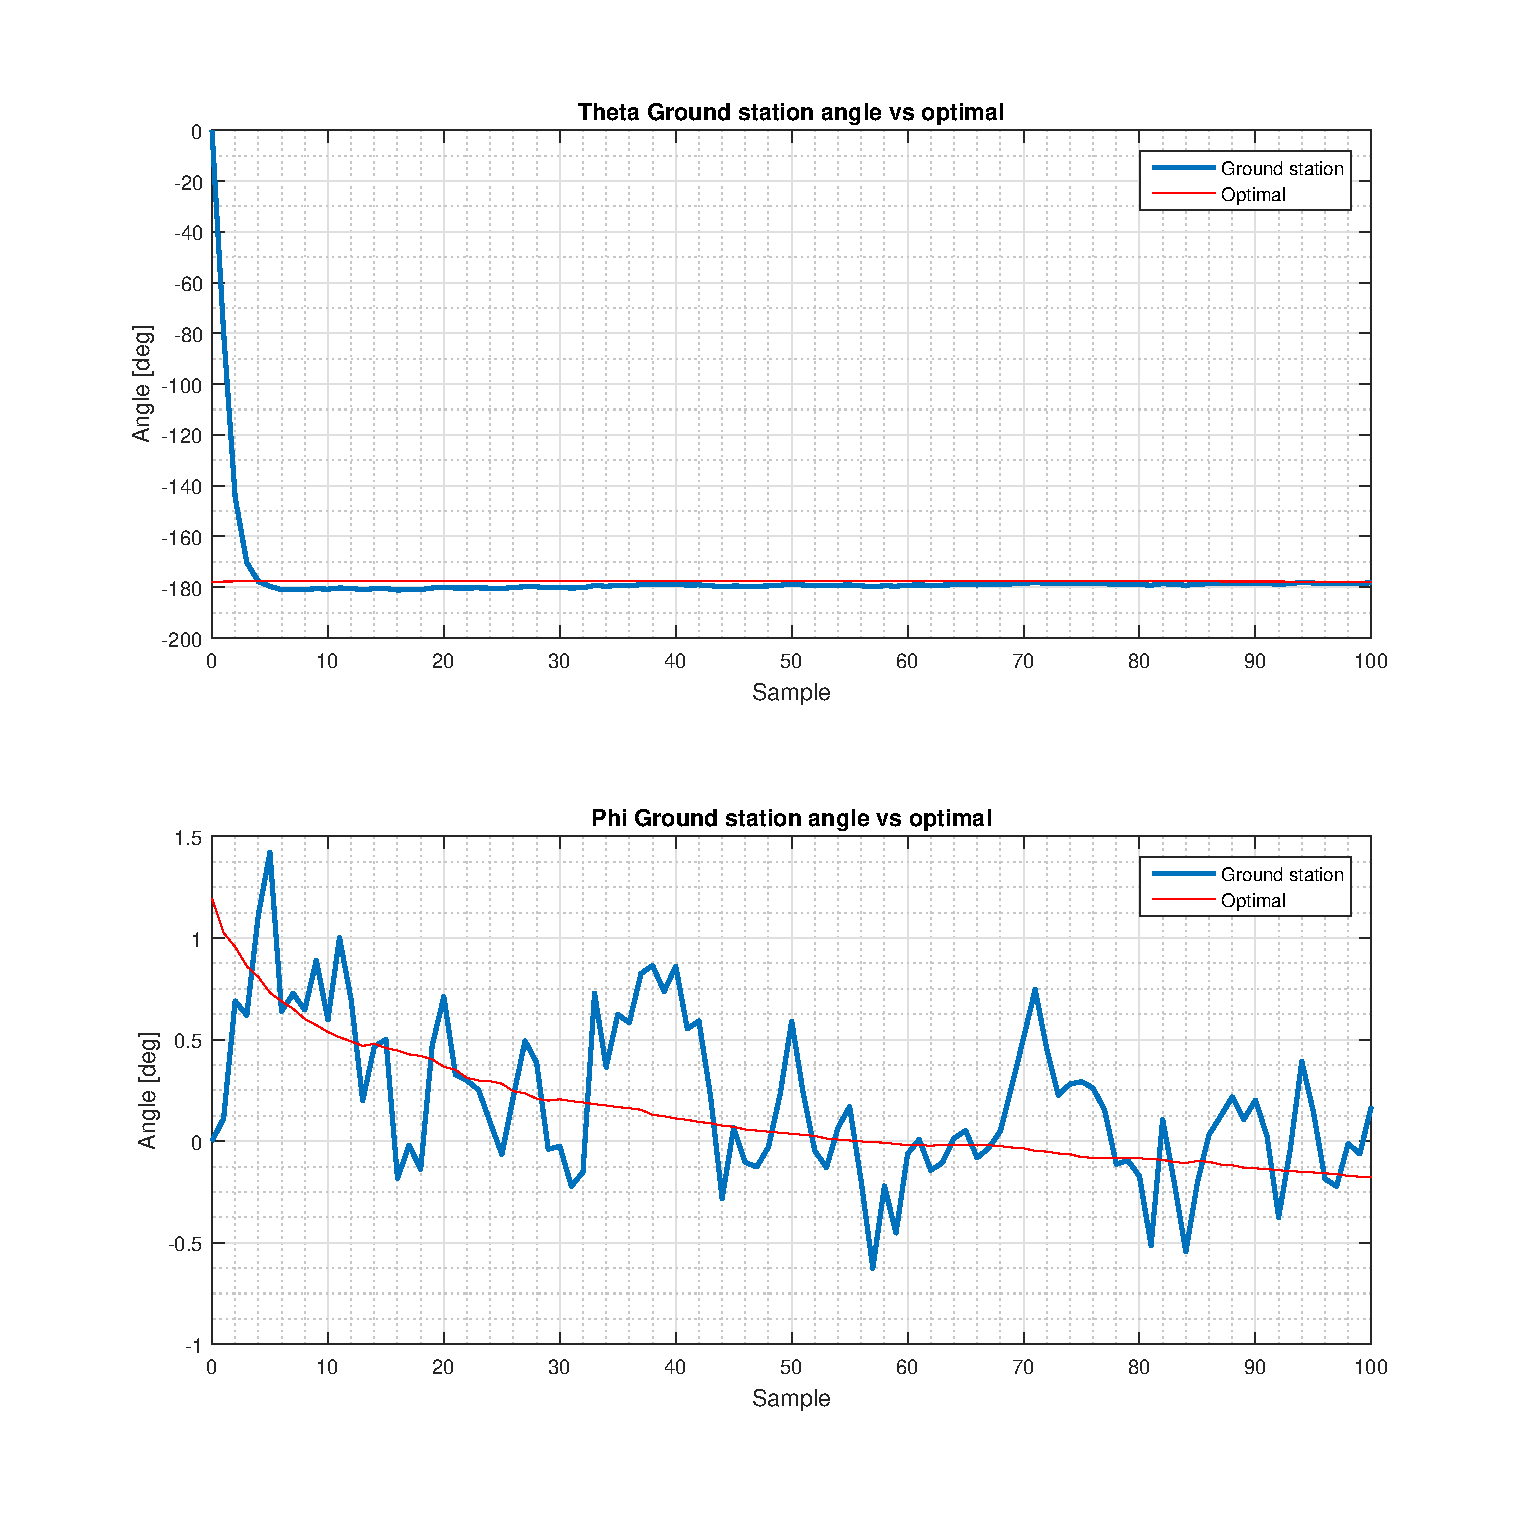
\includegraphics[width=\linewidth]{figures/s2_pi_gs_theta_phi_optimal.eps}
\caption{pi}
\label{fig:s2_gs_pi}
\end{minipage}

\vspace*{0.5cm} % (or whatever vertical separation you prefer)
\begin{minipage}[t]{0.45\textwidth}
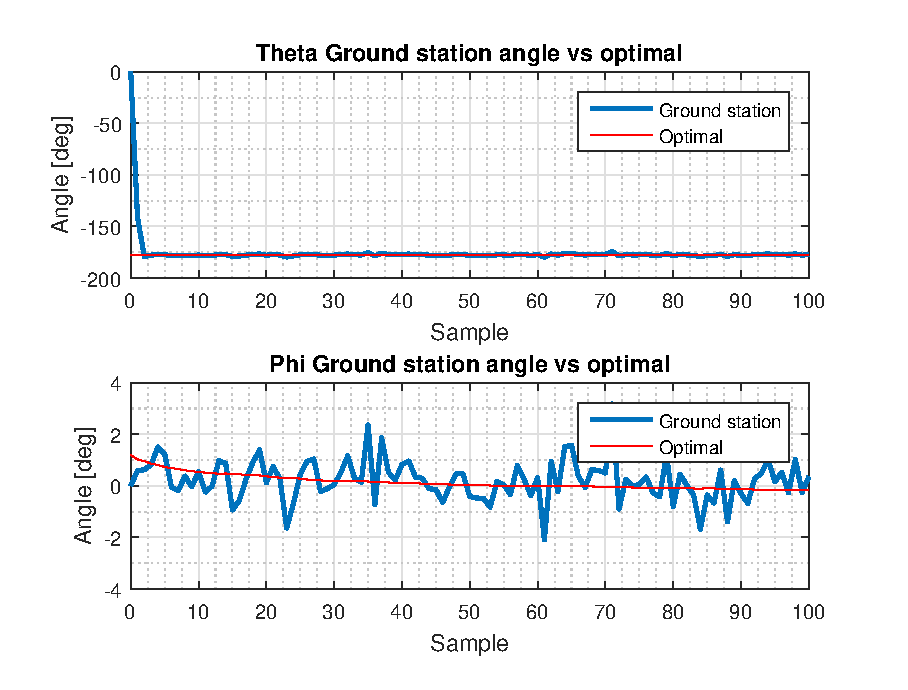
\includegraphics[width=\linewidth]{figures/s2_pd_gs_theta_phi_optimal.eps}
\caption{pd}
\label{fig:s2_gs_pd}
\end{minipage}
\hspace{\fill}
\begin{minipage}[t]{0.45\textwidth}
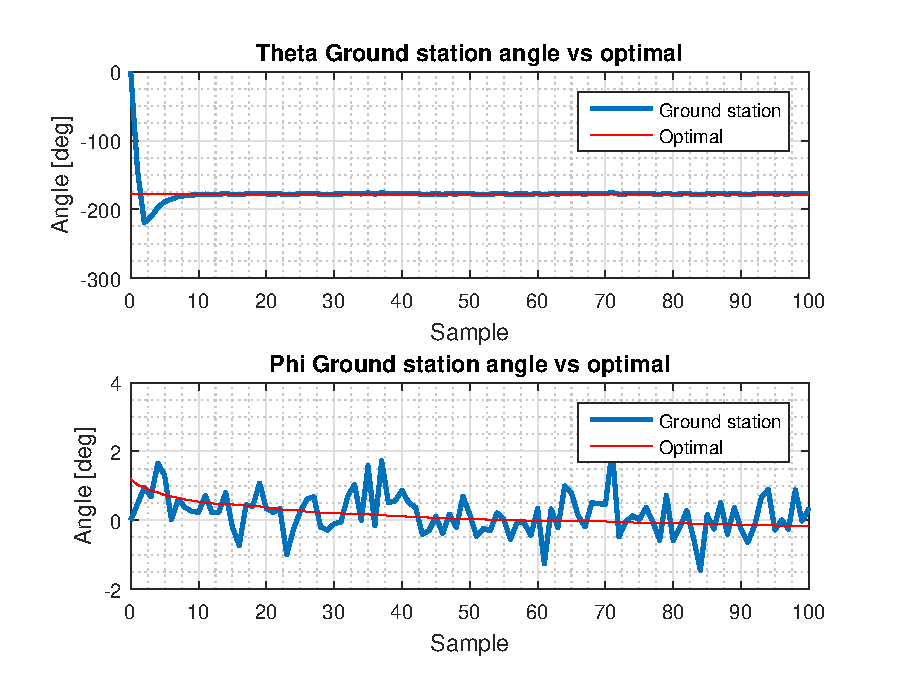
\includegraphics[width=\linewidth]{figures/s2_pid_gs_theta_phi_optimal.eps}
\caption{pid}
\label{fig:s2_gs_pid}
\end{minipage}

\end{figure}

\subsection{prx}
Figure \ref{fig:s2_p_prx}, \ref{fig:s2_pi_prx}, \ref{fig:s2_pd_prx} and \ref{fig:s2_pid_prx}
\begin{figure}[H]
\begin{minipage}[t]{0.45\textwidth}
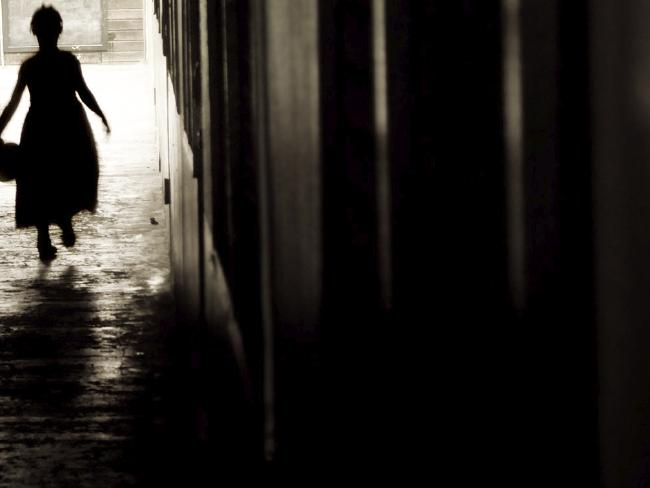
\includegraphics[width=\linewidth]{figures/randomfigure.jpg}
\caption{p}
\label{fig:s2_p_prx}
\end{minipage}
\hspace{\fill}
\begin{minipage}[t]{0.45\textwidth}
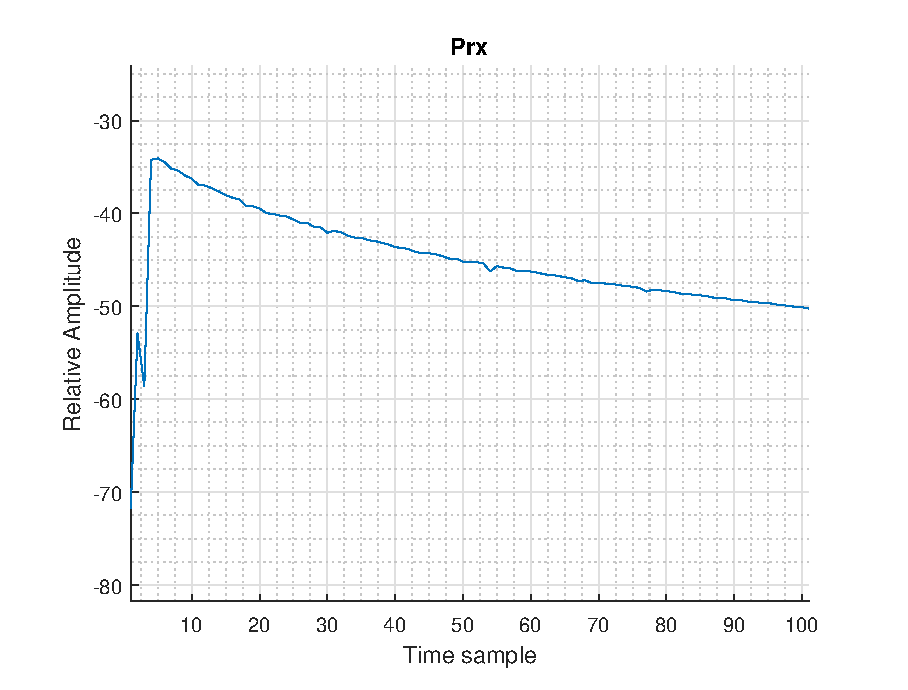
\includegraphics[width=\linewidth]{figures/s2_pi_prx.eps}
\caption{pi}
\label{fig:s2_pi_prx}
\end{minipage}

\vspace*{0.5cm} % (or whatever vertical separation you prefer)
\begin{minipage}[t]{0.45\textwidth}
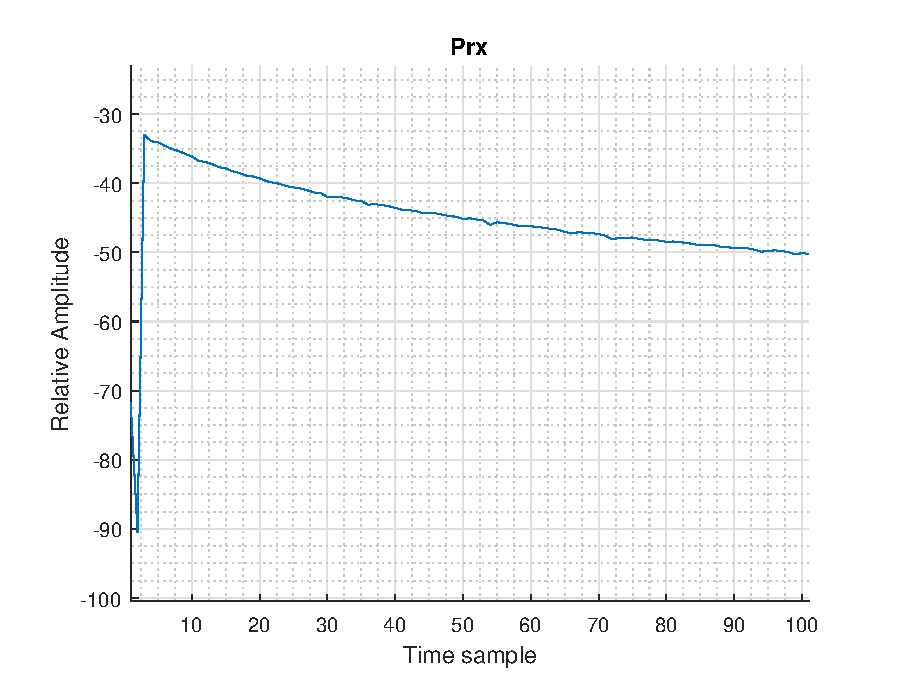
\includegraphics[width=\linewidth]{figures/s2_pd_prx.eps}
\caption{pd}
\label{fig:s2_pd_prx}
\end{minipage}
\hspace{\fill}
\begin{minipage}[t]{0.45\textwidth}
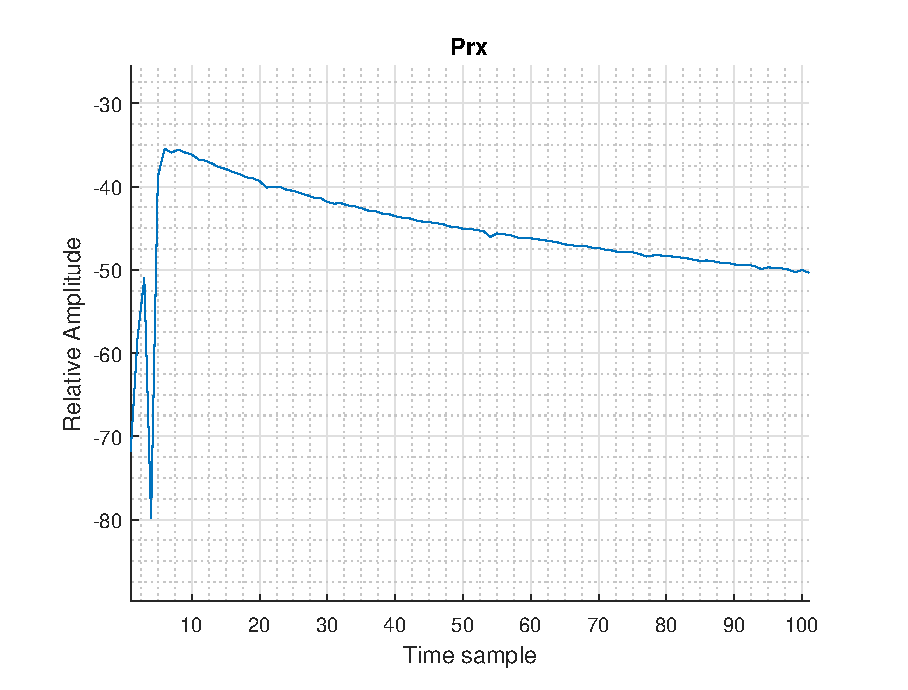
\includegraphics[width=\linewidth]{figures/s2_pid_prx.eps}
\caption{pid}
\label{fig:s2_pid_prx}
\end{minipage}

\end{figure}

%
%\begin{figure}[H]
%\hfill
%\subfigure[.]{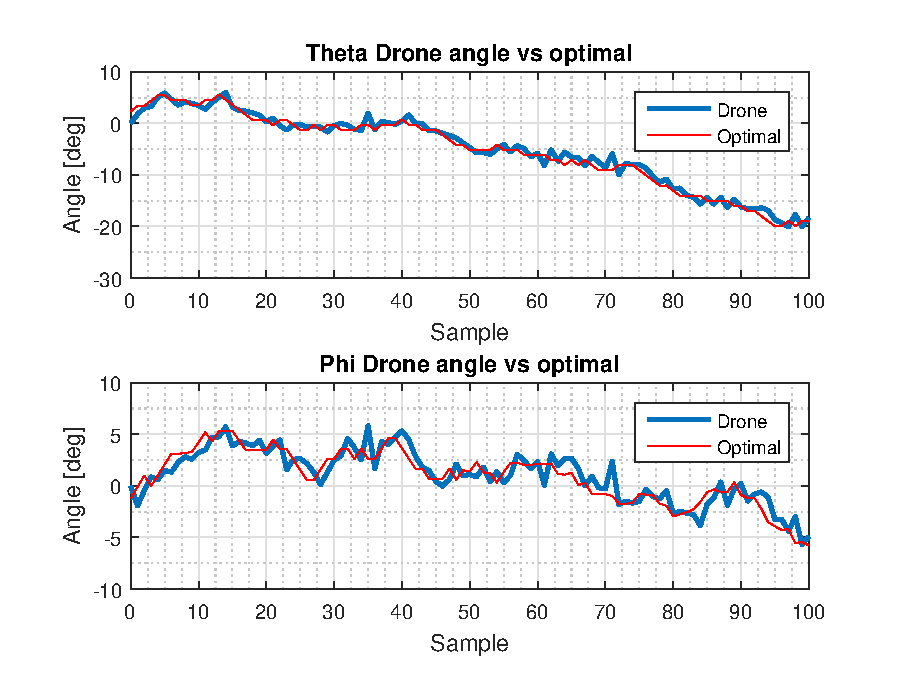
\includegraphics[scale=0.4]{figures/s2_pd_drone_theta_phi_optimal.eps}}
%\hfill
%\subfigure[caption]{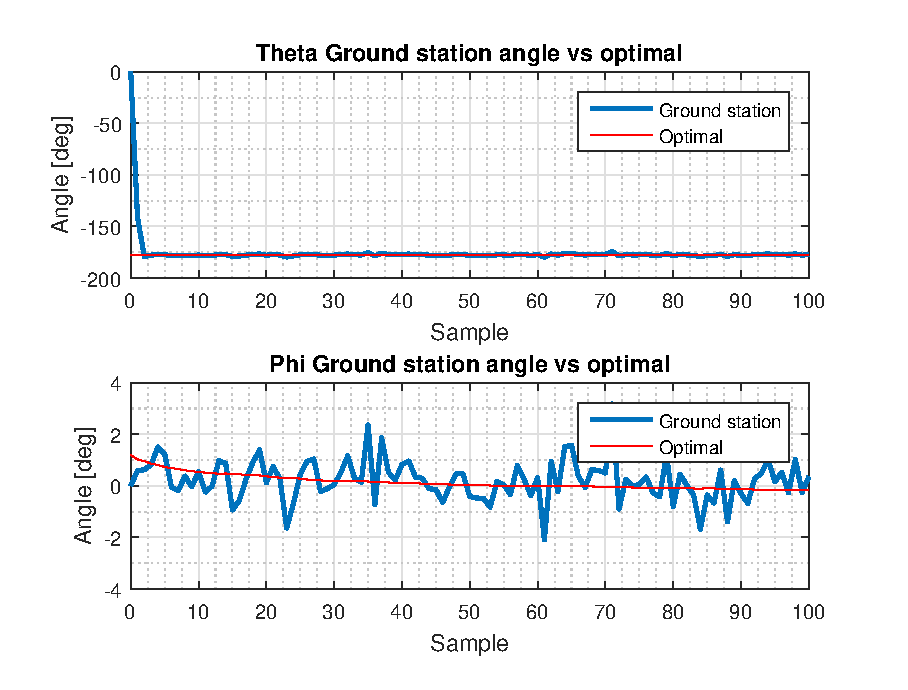
\includegraphics[scale=0.4]{figures/s2_pd_gs_theta_phi_optimal.eps}}
%\hfill
%\caption{caption}
%\label{fig:sinc}
%\end{figure}
%
%\subsection{pd controller}
%
%\begin{figure}[H]
%	\centering
%	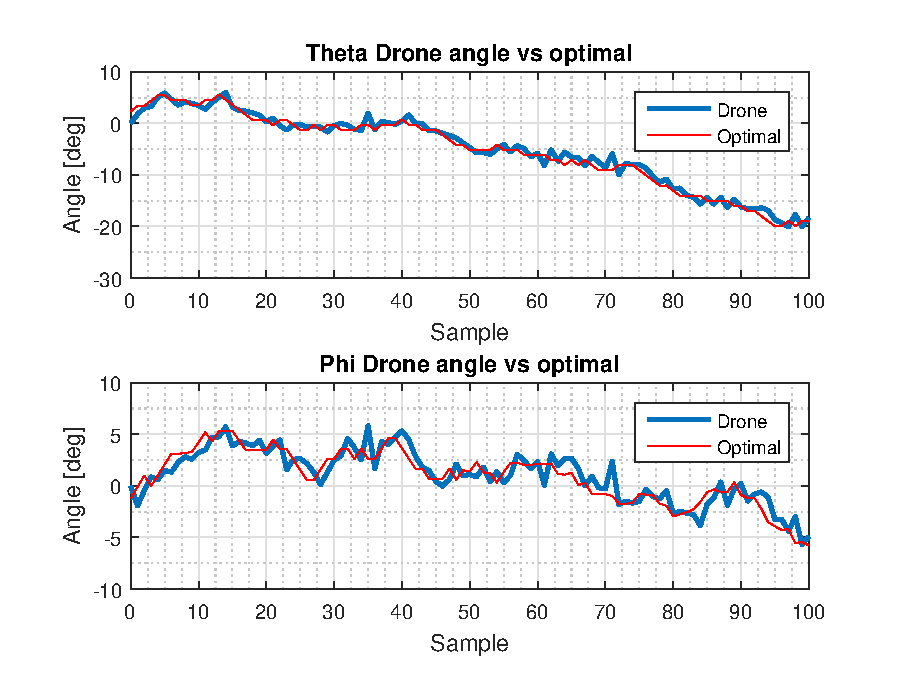
\includegraphics[scale=0.65]{figures/s2_pd_drone_theta_phi_optimal.eps}
%	\caption{}
%\end{figure}
%
%\begin{figure}[H]
%	\centering
%	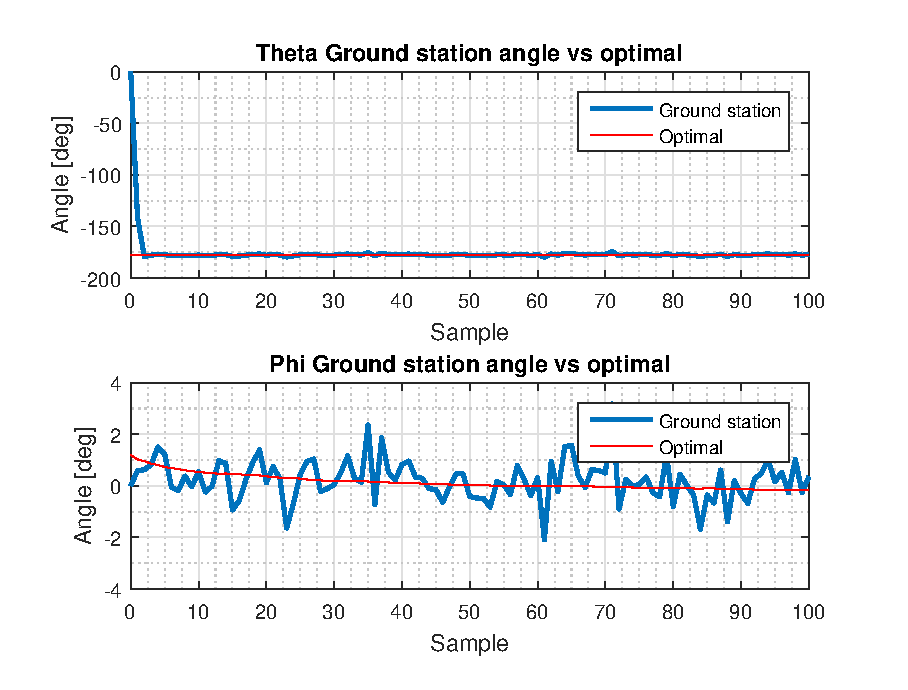
\includegraphics[scale=0.65]{figures/s2_pd_gs_theta_phi_optimal.eps}
%	\caption{}
%\end{figure}
%
%\begin{figure}[H]
%	\centering
%	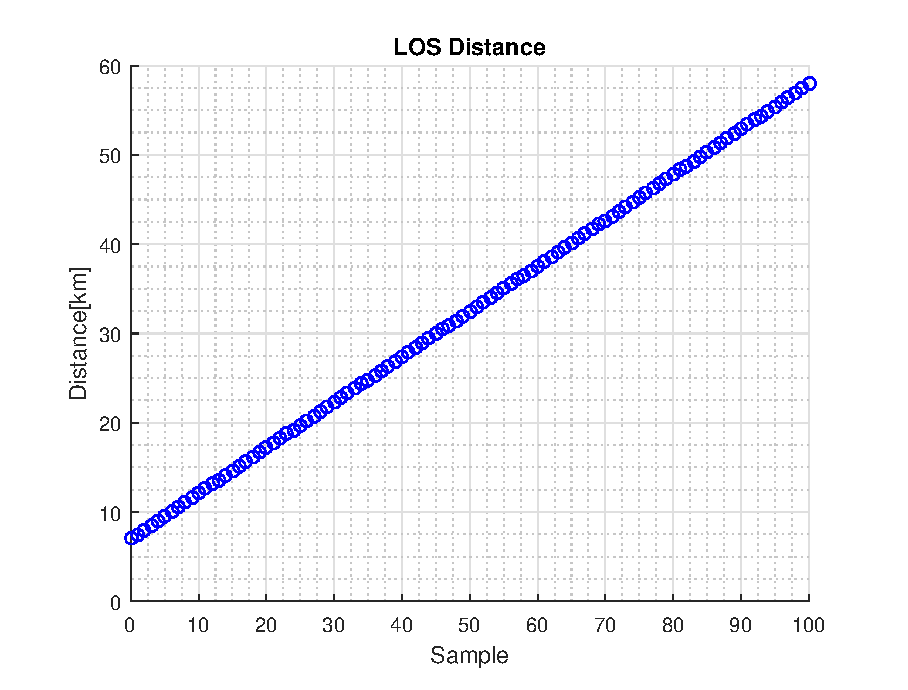
\includegraphics[scale=0.65]{figures/s2_pd_los_distance.eps}
%	\caption{}
%\end{figure}
%
%\begin{figure}[H]
%\hfill
%\subfigure[.]{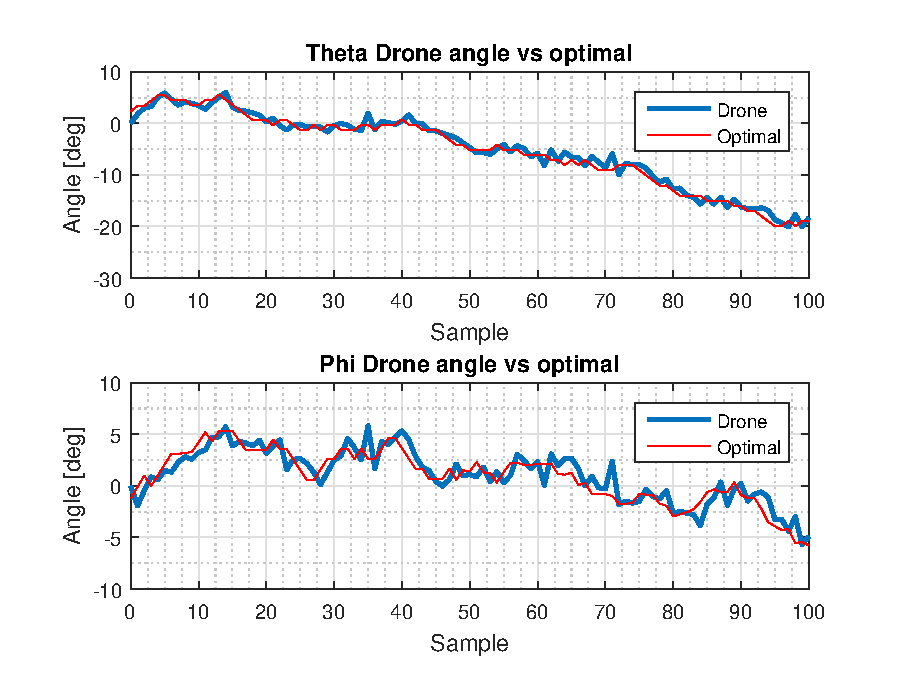
\includegraphics[scale=0.4]{figures/s2_pd_drone_theta_phi_optimal.eps}}
%\hfill
%\subfigure[caption]{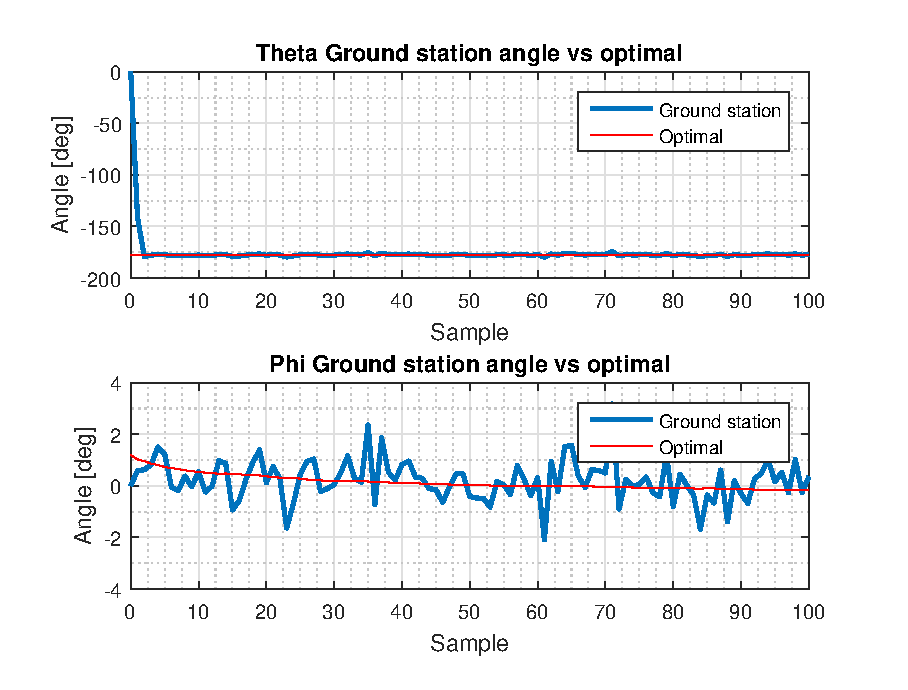
\includegraphics[scale=0.4]{figures/s2_pd_gs_theta_phi_optimal.eps}}
%\hfill
%\caption{caption}
%\label{fig:sinc}
%\end{figure}




